% !TeX spellcheck = en_US
\section{Recording Quality Assessment Algorithms}
\label{sec:554_quality_assessment}
The previous section introduced video-based, auxiliary sensor-based, and hybrid algorithms. 
One major contribution of this work is a first attempt to introduce hybrid algorithms, which adapt and fuse input from different sensors to improve reliability and decrease runtime.
\subsection{Quality Assessment Stages}
\label{sec:554_QA_Algorithms}
Figure~\ref{fig:554_Overview_Stages_crop} shows the various stages of processing in a quality assessment algorithm.
The steps can be classified into
\begin{itemize}
\item access of sensors, 
\item the control stage, which makes an adaptation decision based on sensor samples\footnote{This may involve processing of the sensor values in order to make an adaptation decision.} and synchronizes multi-sensor input, 
\item the algorithm stage, in which the algorithm processes data from the sensors, and 
\item the model stage, which generates the quality score.
\end{itemize} 
The different stages of algorithm processing are described in the remainder of this chapter.
\begin{figure}[!htb]
\centering
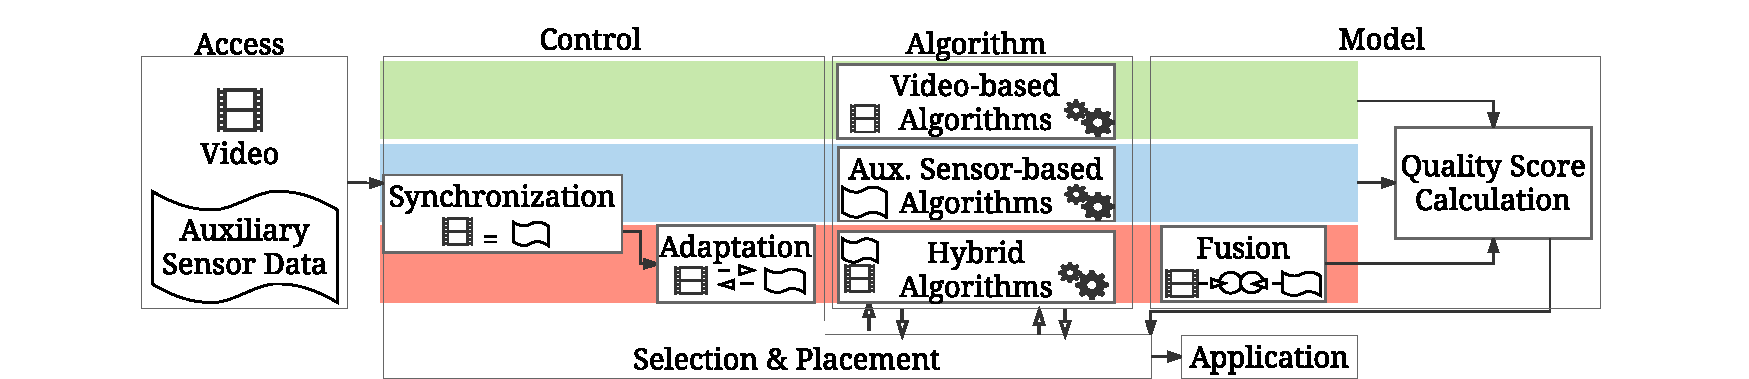
\includegraphics[width=\linewidth]{./gfx/550_QA/Overview_Stages_crop}
\caption{Different processing stages running a quality assessment algorithm}
\label{fig:554_Overview_Stages_crop}
\end{figure}
\subsubsection{Access}
The access stage is responsible for retrieving sensor input. Sensors can be the camera for video-based algorithms, the microphone of the recording device for an audio analysis, and any other auxiliary sensor in a mobile device, e.g., accelerometer or gyroscope.

As soon as the device offers a new sample, it is received in the access stage.
Many algorithms store a series of sensor inputs because they need a temporal assessment. % over a sample\textit{window}. 
A window of samples is used for $n$ frames in video-based, or $n$ sensor samples in auxiliary sensor-based algorithms.
In these cases, the access stage acts as a buffer before invocation of the algorithm stage.
Hybrid algorithms access multiple sensors simultaneously and invoke the processing of sensor samples.
Note that the synchronization of sensor samples with video frames can be realized by the algorithm or the control stage.
\subsubsection{Control}
\label{sec:554_Control}
The control stage is responsible for the coordination of the quality assessment (see Figure~\ref{fig:554_Overview_Stages_crop}).
It is in charge of synchronizing different sensor inputs, i.e., for auxiliary sensor-based algorithms or hybrid algorithms.
As the samples of various sensors are not automatically in sync, synchronization is required to ensure that quality scores that leverage different inputs can be precisely mapped to the media. 

Synchronization of the different sensor streams is achieved on a device using the system clock timestamps. 
During a recording session, drifts in timestamps may occur due to delays of the physical sensors as well as due to the operating system that offers the samples~\cite{Guggenberger2015}. 
Related work has shown that during a recording session this drift may add up to a maximum of $19$ milliseconds per hour of recorded videos for recent smartphones such as the LG Nexus 4 and the LG Nexus 5. 
This drift is negligible, as even for the different modalities of audio and video, a human-perceivable difference occurs at a drift of around $\pm 80$ milliseconds~\cite{Steinmetz1996}. % is perceived as synchronized~\cite{Steinmetz1996}.
\paragraph{Adaptation}
\label{sec:554_Adaptation}
An adaptation between sensors is beneficial if the single sensor algorithms perform differently for different environmental conditions.
An adaptation of a hybrid algorithm is applied to either ensure high precision at any time or reduce the runtime at a given precision.
Auxiliary sensor signals can be used to determine when environmental conditions are good for applying video-based analysis.
For \ac{UGV} quality assessment, Bano et al. showed that the precision of video-based quality assessment algorithms suffers from significant luminance variations~\cite{Bano2015}.
This finding can be mapped to an adaptation rule to determine if a video-based algorithm is suitable for searching degradations in a video.
We determine the sensed lighting around a device for an approximation of the luminance in the video:
\begin{equation}
\label{eq:554_luma_threshold}
V_{j,w_i} = \begin{cases}
1,& \text{if } L_{w_i}(j) \geq T_{L,D}\\
0,& \text{otherwise}
\end{cases}
\end{equation}
Here, $V_{j,w_i}$ represents a binary indicator - whether the video-based algorithm shall be considered for a specific video frame $j$ in the sample window $w_i$.
$L_{w_i}(j)$ depicts the average light intensity for $j$ in window $w_i$.
It is determined by samples from the light sensor in a smartphone. 
A decision on if a video-based algorithm can be applied for quality assessment is based on whether the majority of the frames in $w_i$ fulfill $V_{j,w_i} = 1$ or not. 

$T_{L,D}$ is a device-specific threshold as the sensed samples vary significantly between manufacturers of the light sensors embedded in smartphones~\cite{Bano2015}.
For example, the LG Nexus 4 shows good ambient light conditions at around $100.0$ $ \unit{lx}$, whereas under the same conditions a Samsung Galaxy S2 senses around $20.0$ $\unit{lx}$.
The values were gathered based on the video and sensor dataset of Bano et al.~\cite{Bano2015}.

If a recording device does not offer ambient light sensor values, an image-based algorithm is applied.
First, the \textit{RGB} image is converted into a \textit{YUV} representation. 
Here, $Y$ represents the luma plane and the other two are chrominance ($UV$) planes. 
The planes are split, and solely the $Y$ component is used as it depicts the luma intensity. 
The light intensity per frame is calculated as
\begin{equation}\label{eq:554_lumaip}
\mathcal{L}_{j} =\frac{1}{N_r*N_c} \displaystyle\sum_{k=1}^{N_r} \displaystyle\sum_{l=1}^{N_c} Y_{I}(k,l)
\end{equation}
Here, $\mathcal{L}_{w_i}(j)$ represents the average luma intensity of the luma plane ($Y_I$) of frame $j$.
$k$ and $l$ represent the pixel coordinates, where $N_r$ gives the height (rows) of a frame and $N_c$ the width (columns).
Based on the average luma intensity of a frame, it is determined if an image processing algorithm should be used.
\begin{equation}
V_{j,w_i} = \begin{cases}
1,& \text{if } \mathcal{L}_{w_i}(j) \geq T_{L}\\
0,              & \text{otherwise}
\end{cases}
\end{equation}
Here, $T_{L}$ is the intensity threshold which ensures a good ambient lighting. 
In the parameter study of this work, it is shown that $T_{L} = 50$ offers the best results (see Section~\ref{sec:556_parameters}).
\subsubsection{Algorithm Execution}
\label{554:sec_Algorithm_Execution}
The algorithm execution stage is the execution environment for different quality assessment algorithms, which differ regarding the sensors used.
The algorithms significantly differ regarding precision and runtime.
As a platform for running the algorithms the programming language Java with its Runtime Environment is available for both server and mobile devices.
\ac{JNA} is used for the invocation of native code to be build specifically for operating systems.
The proposed algorithms have been implemented using C, as they are executed significantly faster on mobile devices, e.g., for an LG Nexus 5 between 2.2 to 17.8 times faster\footnote{http://www.learnopengles.com/a-performance-comparison-between-java-and-c-on-the-nexus-5/; Visited on: 07/20/2016}.

According to their input signal, algorithms are classified into video-based, auxiliary sensor-based and hybrid ones. 
As they differ in their respective input, they may also differ regarding their results.
The model stage is responsible for mapping the algorithm results to a uniform quality value, which can then be used by the application requesting the quality assessment.
\subsubsection{Model Stage}
\label{sec:554_model_stage}
The model stage is responsible for calculating the quality value  for all algorithms. 
A common step for any algorithm represents the mapping of its result to the \ac{MOS}.
The findings of Chapter~\ref{chapter:400_RecordingQuality} are used to calculate the \ac{MOS} for the degradations: camera shake, harmful occlusions, and camera misalignment.
The proposed algorithms do not only depict, if a degradation is present, but also quantify their impact; e.g., for a camera shake by depicting the direction, speed, and amplitude of the shake.
The calculated result is sent to the application that initially requested the quality assessment. 

For hybrid algorithms the model stage is also responsible for fusing results provided by subalgorithms. Hybrid algorithms analyze inputs from different sensors in different subalgorithms.
Instead of relying on only one sensor, the combination of results derived from multiple sensor inputs can improve the precision~\cite{Cricri2012}. 
An algorithm designer can decide when to calculate a fused score $S_{V,AS}$:
\begin{equation}
S_{V,AS} = o_{V} \times S_{A_{V},w_{i,V}} + o_{AS} \times S_{A_{AS},w_{i,AS}}
\end{equation}
Here, $o_{V}$ represents the weight for the degradation score calculated by the video-based algorithm, and $o_{AS}$ the score based on auxiliary sensors. 
The weights $o_{V}$ and $o_{AS}$ are normalized between $[0, 1]$, and the condition $o_{V} + o_{AS} = 1 $ must hold.
$w_{i,AS}$ and $w_{i,V}$ represent the auxiliary sensor sample window and the video frame window used in the algorithm execution stage.
Algorithms use the fusion of the algorithm output when subalgorithms present contradicting results.

In the remaining subsections, algorithms for detecting and quantifying degradations are given for camera shakes, harmful occlusions, and camera misalignments.   
% -  -  -  -  -  -  -  -  -  -  -  -  -  -  -  -  -  -  - --
\subsection{Camera Shake Assessment}
\label{sec:554_QA_Camera_Shakiness}
Chapter~\ref{chapter:400_RecordingQuality} has shown that camera shakes reduce the perceived quality of a video. As no reliable algorithm exists to quantify its impact, it is proposed to have an auxiliary sensor-based algorithm, a video-based algorithm, and a hybrid algorithm combining the two.
\subsubsection{Auxiliary Sensor-based Algorithm}
The identification of camera shakes during recording is based on the three-dimensional linear accelerometer sensor.
It offers a fine-grained measurement of the acceleration without gravity components in $\frac{m}{s^2}$ on three axes. 
For the camera shake assessment, a window of $m$ samples is used to monitor the device motion.
The definition of a small sample window is based on the work on camera tilts and panning by Cricri et al.~\cite{Cricri2012}. 
To reduce the computational burden, the linear accelerometer gathers a subset of $15$ samples ($f=15$ $\unit{Hz}$) in a window of one second.
A low-pass filter is applied to reduce the window size and avoid noise generated by the sensitive sensors\footnote{The low-pass filter uses a threshold of $\alpha = 0.3$ and iterates linear accelerometer samples $a$ with index $i$ by applying $a_i=a_{i-1} + \alpha * (a_{i} - a_{i-1} )$.}.
In contrast to camera tilts and pans, shakes can be identified by at least two consecutive direction changes. 
The number of direction changes is measured by the counter $c_{d}$. 
If no movement is measured for the sample size $m$, the counter $c_{d}$ is reset. 
The resulting algorithm (see Algorithm~\ref{algo:554_shake}) illustrates how a camera shake can be detected based on direction changes.

\begin{algorithm}[!h]
	\caption{Proposed algorithm for the detection of camera shakes based on the linear accelerometer.}
	\begin{algorithmic}
		
		\Require \textbf{function} \textbf{sgn}($p$,$q$): 3D-Signum-Function - calculates the sign of the difference of $p$ to $q$ for each dimension of a 3D vector and returns a 3D vector.
		\Require \textbf{function} \textbf{MAX}($p[]$): Calculates highest absolute acceleration in the array $p[]$ of three-dimensional vectors
		\Require \textbf{Require:} $s[]$: Three-dimensional sample array (x,y,z) of size $m$ filled with linear accelerometer sensor samples
		\Require \textbf{Require:} $t$: Latest sample index
		\Require \textbf{Require:} $T_{S,AS}$: Threshold for identifying significant camera shake
		
		\State $c_{d} \gets 0 $
		\If {$s_{t, x} \neq s_{t-1, x}$ \Or $\, s_{t, y} \neq s_{t-1, y}$ \Or $\, s_{t, z} \neq  s_{t-1, z} $}
		\For {$i \gets 0 .. t-3$}
		\If{$sgn(s_{i},s_{i+1}) \neq sgn(s_{i+1},s_{i+2})$}
		\State 	$c_{d} \gets c_{d} + 1 $
		\EndIf
		\EndFor
		\If{$c_{d} \geq 2 $ \textbf{and} $ max(s[]) \geq T_{S,AS}$}
		\State \Return $true$
		\EndIf 
		\EndIf
		\State \Return $false$
	\end{algorithmic}
	\label{algo:554_shake}
\end{algorithm}

A detected camera shake in a window of $m$ samples is used to determine not only if a shake is present but also to which extent it degrades the perceived quality.
The speed (frequency) and amplitude of camera shakes are calculated on the basis of the directional changes.
The algorithm applies a signum function to determine the direction of linear accelerometer values. 
To compensate small and imperceivable changes, a threshold $T_{S,AS}= 0.2\frac{\unit{m}}{s^2}$ determines the minimum acceleration for a harmful shake. 

Besides this classification, a quantification is also possible solely relying on $\frac{c_{d}}{l(w_{i})} \unit{\frac{1}{s}}$, by calculating the frequency of the shake.
Here, $l$ depicts a length function for retrieving the window size and $c_{d}$ gives the counter of direction changes. 
The amplitude of a camera shake is determined by the time a camera movement into a specific direction is detected by measuring both a dense window of samples from the linear accelerometer ($> \frac{16}{s}$) and the corresponding timestamps for the readings.
The sample window is iterated to compute the average acceleration in each direction until a direction change is detected.
Then the distance into a specific direction is computed as $D = \Delta t^2 * \overline{LA(x,y,z)} [\unit{m}] $, where $\Delta t$ represents a continuous movement about a specific axis measured in $[\unit{s}]$ and $\overline{LA(x,y,z)}$ depicts the linear accelerometer values\footnote{A calibration of the device is needed with approximately 100 samples to reliably determine the individual white noise of gyroscope and accelerometer.}.
A mapping is still needed for the camera model to map the distance in meters to pixels that were crossed in a given window.
This mapping is based on an initial calibration step, e.g., when a new device runs the quality assessment for the first time. 
A combined analysis of the correlation of different linear accelerometer samples to pixel movements is performed using a Canny filter~\cite{Canny1986}.
After this initial calibration and synchronization step, no video-based techniques need to be applied.
The determined influence factors are then mapped to the formula known from Chapter~\ref{chapter:400_RecordingQuality} to determine the \ac{DMOS} as
$\Delta MOS = 0.8739 * x_{amplitude} + 0.0682  * x_{time} + 2.961 * x_{speed}$, or the respective genre-dependent coefficients. 
The \ac{DMOS} determines the absolute quality loss induced by a camera shake. 
\subsubsection{Video-based Algorithm}
The video-based algorithm for camera shake detection performs a global motion analysis between the two video frames represented as intensity matrices.
Based on this analysis, repetitive changes in motion are classified as camera shakes.
Figure~\ref{fig:554_CSAlgorithm} gives an overview of the algorithm.
In a window of $N$ video frames, the algorithm extracts two consecutive video frames per iteration.
A fast intensity-based approach is used that is based on the \ac{FSGPA}~\cite{Hao2013}.
For detecting motion, $64\times64$ pixel subblocks of the intensity representations are extracted from each video frame.
The subblock detection or sifting step filters subblocks whose average intensity per pixel is below $T_{lowGray} = 98$ (see Section~\ref{sec:556_parameters}). 
All subblocks with such a low-intensity are not considered for motion calculation.
The rationale behind this step is that motion cannot be reliably determined in low-intensity frames.
 \begin{figure}[!htb]
 	\centering
 	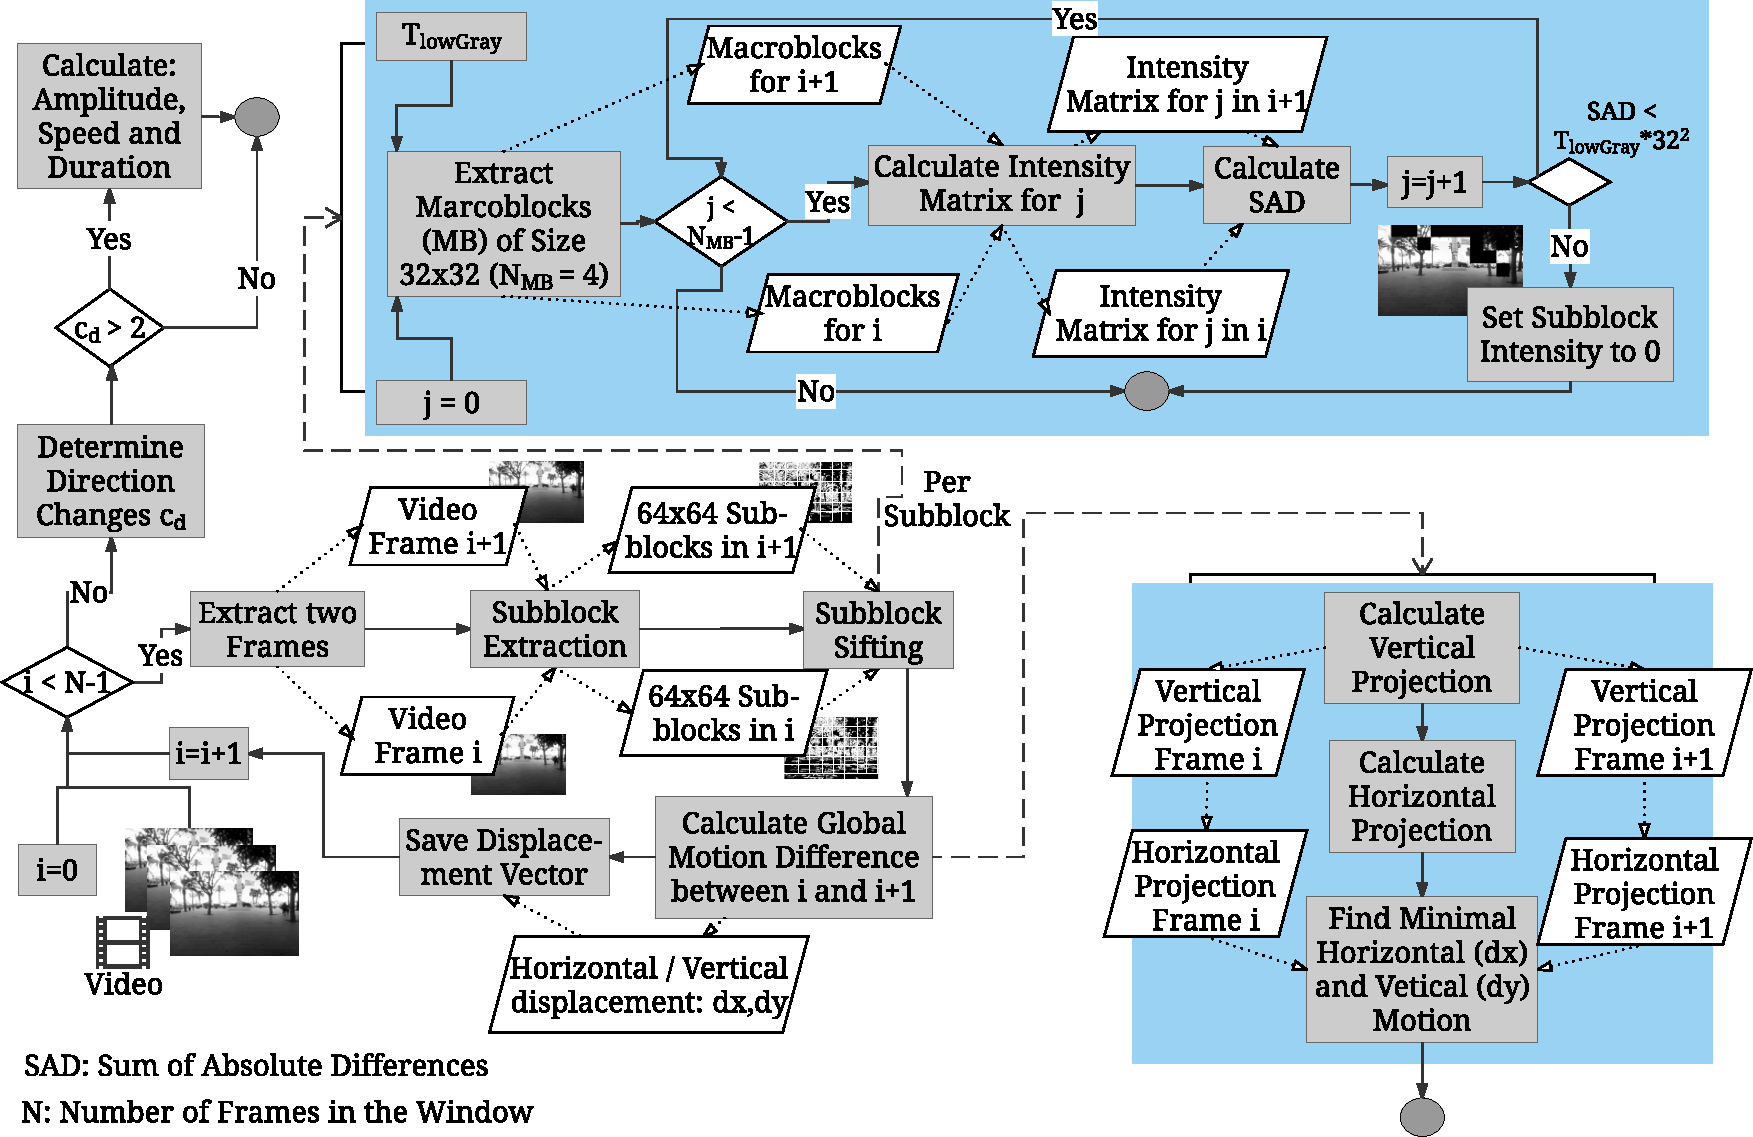
\includegraphics[width=\linewidth]{./gfx/550_QA/Camera_shake_algorithm_Video_based}
 	\caption[Flow chart of the video-based camera shake detection algorithm]{Flow chart of the camera shake detection algorithm, relying on a video-based detection of motion in the horizontal and vertical plane. The blue boxes detail essential steps in the process. Pictures illustrating video frames are taken from the \textit{CMDG} dataset~\cite{Bano2015}.}
 	\label{fig:554_CSAlgorithm}
 \end{figure}
 
The global motion between two filtered frames is estimated by analyzing the horizontal and vertical projections of a video frame independent of each other.
Vertical and horizontal motion vectors are determined by finding the minimal, common movement of all subblocks - indicated by a minimal error when mapping the two intensity frames. 
In a search breadth of $m = 1$ for each subblock, it is determined whether it has moved up to $2 * m + 1$ blocks.
The minimum of the \ac{SAD} indicates the steps a subblock has moved, i.e., in the horizontal and vertical translation:
\begin{equation}\label{eq:554_mvs}
d_x = m + 1 - w_{min, h} \text{, } d_y = m + 1 - w_{min, v}
\end{equation}
Here, $w_{min, h}$ indicates an alignment to compensate for motion in the horizontal direction.
Similarly, $w_{min, v}$ indicates the vertical alignment.
Based on this motion estimation, the number of direction changes can be determined.
The motion estimation is recalculated for all entries in a window of video frames.
As soon as at least two direction changes are detected, a camera shake is identified.
Using methods proposed by Saini et al. and Campanella et al., pan, tilt, and shake can be distinguished using a median or low-pass filter on the motion vectors $d_x$ and $d_y$~\cite{Campanella2007,Saini2012}. 
The \ac{SAD} is computed between the original and filtered motion vectors. 
The absolute differences of the intensity values are summed to determine a shake score in the range of $[0, 1]$.
$S_{S, V}$ represents a shake score that is determined based on the calculated \ac{SAD} in the vertical and horizontal projection of the video frames:
\begin{equation}
 S_{S, V} = \sqrt{{SAD_{h}}^2 + {SAD_{v}}^2}
\end{equation}
 Based on the $T_{S,V}$ a shake can be distinguished from an intended pan and tilt.
 If the detected score is above this threshold, the motion is classified as shake.
 This condition triggers the calculation of the amplitude, speed, and duration of a camera shake.
 Similar to the auxiliary sensor-based camera shake detection, the findings of our subjective analysis can be used to determine the degradation impact by calculating the \ac{DMOS} as $\Delta MOS = 0.8739 * a_{ampl} + 0.0682  * a_{dur} +  2.961 * a_{speed}$.
%================================================================================================================
%====================================== OCCLUSION ===============================================================
%================================================================================================================ 
\subsection{Harmful Occlusion}
\label{sec:554_QA_Harmful_Occlusion}
%Despite intensive research the sensors available in retail smartphones, such as lasers for auto focus detection or proximity sensors used for distance calculation are not yet capable for reliably supporting harmful occlusion detection.
Video-based algorithms are proposed to detect and assess harmful occlusions.
Additionally, a contribution towards the design of adaptive video-based algorithms for harmful occlusion detection in \ac{UGV} is made.
Auxiliary sensors are used to determine when to switch between the video-based algorithms.
\begin{figure}[!htb]
	\centering
	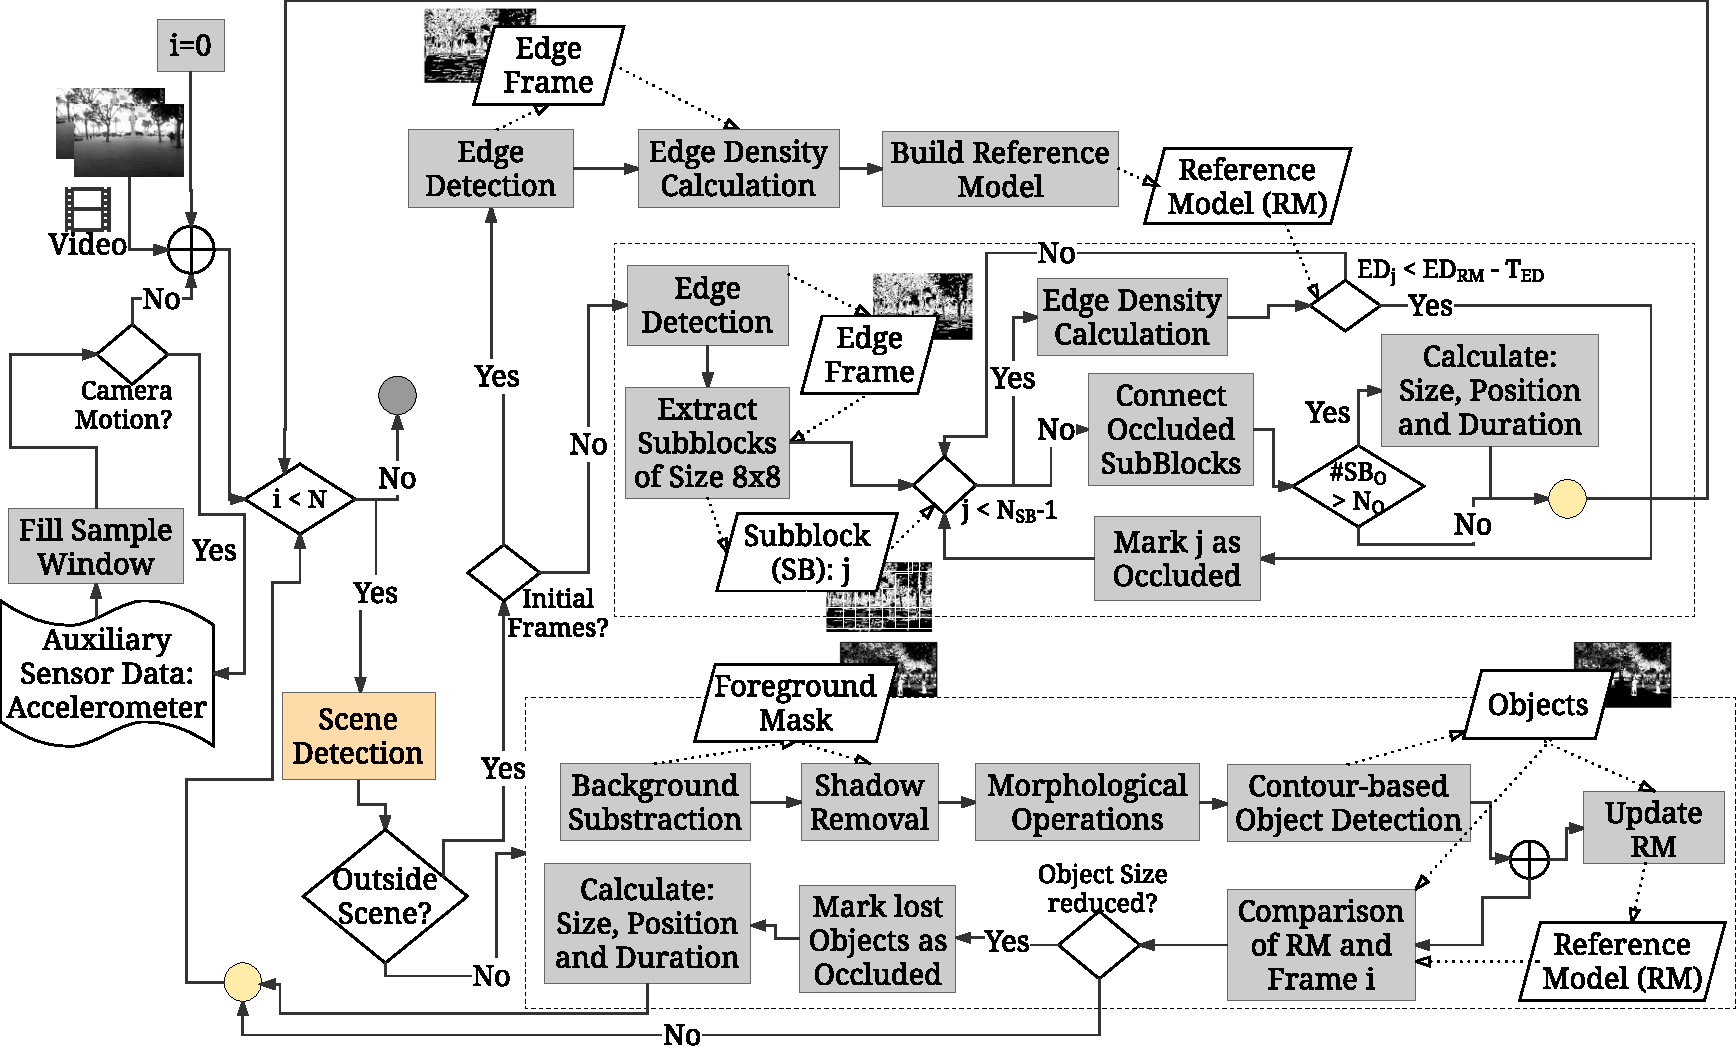
\includegraphics[width=\linewidth]{./gfx/550_QA/Occlusion_Algo}
	\caption[Video-based harmful occlusion detection algorithm]{Overview of the proposed occlusion detection algorithm showing the video-based calculation and its auxiliary sensor-based adaptation.}
	\label{fig:554_Occlusion}
\end{figure}
\subsubsection{Edge Density-based Occlusion Detection}
The proposed approach extends the research of Saini et al., who proposed to calculate the edge density of video frame patches~\cite{Saini2012}.
A harmful occlusion requires that an occluding object must be closer to the camera than the recorded \ac{AoI}.
In a two-dimensional video frame representation, an object being recorded at a close distance to the camera lense has a higher average distance between the object's contour pixels than the contour pixels of the same object at a larger distance to the camera.
When tracking a pixel block in a video over time, a sudden increase of the edge distances indicates a possible occlusion.

The process of detecting these occlusions is shown in Figure~\ref{fig:554_Occlusion}, which calculates an edge density for consecutive video frames in different blocks of size $8\times8$.
After detecting edges using the Canny edge filter~\cite{Canny1986}, the edge density is calculated using the edge frame and convoluting it with a $3\times3$ unity matrix of ones.
This step strengthens edges present in the video frame.

The edge pixels are counted per subblock:
\begin{equation}
ED_{j} = \sum_{i=1}^{N_r}\displaystyle\sum_{k=1}^{N_c} SB_{I} (i,k)
\end{equation}

Here, $j$ iterates over all subblocks of size $8\times8$, and $i$ and $k$ depict the indices for the subblock pixels.
For each subblock $j$, the edge density $ED$ is calculated by summing the intensity $SB_I$.  
As soon as a block's edge density $ED_j$ falls below $ED_{RM} - T_{ED}$, the subblock is labeled as being harmfully occluded.
This threshold helps to separate structures with a low-edge density from harmful occlusion candidates as the edge density must significantly drop from a reference value. 
These objects, containing low-edge densities, would otherwise be classified as harmful occlusions.
Also, to fill small gaps in occluded areas, a connected component analysis is performed.
Each non-occluded subblock is labeled as being occluded, if all neighboring subblocks indicate an occlusion.  
\subsubsection{Object Tracking-based Occlusion Detection}
The second algorithm applies occlusion detection by tracking foreground objects.
It relies on a background-to-foreground segmentation.
A foreground mask detection algorithm proposed by Zivkovic et al. is used and improved for \ac{UGV} with a shadow removal technique applied as proposed by Saravanakumar et al. to remove contours from the video frame which do not belong to objects being tracked~\cite{Saravanakumar2012,Zivkovic2006}.
This approach significantly reduces the false classification rate.
It applies a normalized cross-covariance calculation to the frame to detect shadows.
If shadow candidates reach a normalized cross-covariance of 50,\footnote{Determined as an optimal threshold in our parameter study.} they are classified as shadows and are removed from the frame.
This approach requires that a foreground model exists, which is achieved by using Zivkovic et al.'s approach~\cite{Zivkovic2006}.
Background objects in a certain distance are smaller than objects closer to the recording camera.
Thus, when applying a contour filter to a frame, the area with background objects is assumed to be small in comparison to foreground objects.
The results of applying the shadow and background removal are depicted in Figure~\ref{fig:554_des:bs}.
\begin{figure}[!htb]
	\centering
	\subfloat[Original frame with occlusion]
	{\label{fig:des:bs:a}%
		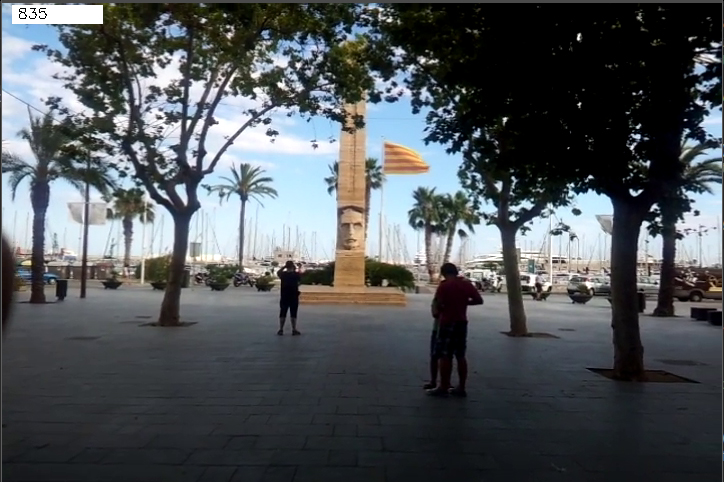
\includegraphics[width=.35\linewidth]{./gfx/550_QA/obj/org_835_fd.jpg}} \quad
	\subfloat[Foreground mask by frame difference method]
	{\label{fig:des:bs:b}%
		\includegraphics[width=.35\linewidth]{./gfx/550_QA/obj/bs_835_fd.png}} \\
	\subfloat[Original frame with occlusion]
	{\label{fig:des:bs:c}%
		\includegraphics[width=.35\linewidth]{./gfx/550_QA/obj/org_835_bs.png}} \quad
	\subfloat[Foreground mask]
	{\label{fig:des:bs:d}%
		\includegraphics[width=.35\linewidth]{./gfx/550_QA/obj/bs_835_my.png}} \\        
	
	\caption[Images show a foreground mask comparison of video frames.]{Foreground mask detection by the frame difference method~\cite{Saravanakumar2012}.} \label{fig:554_des:bs}
\end{figure} 

The remaining foreground frame is compared to a per-frame updated reference model (contours). From the contours, independent objects are detected and counted. An occlusion is assumed, if in the reference model foreground objects cannot be tracked anymore.

The position, size, and duration of an occlusion can then be computed for both approaches in a similar manner and applied to the \ac{MOS} as described in Chapter~\ref{chapter:400_RecordingQuality}. 
The ratio of patches occluded in relation to all patches is then used as the size of the occlusion.
The perceived quality reduction (\ac{DMOS}) is calculated based on the quality model proposed in Section~\ref{sec:430_results_recording_degradations}. 

In comparison to the other algorithms presented in this chapter, the harmful occlusion detection is computational intensive as all subalgorithms rely on video analysis.
The video composition application described in Chapter~\ref{chapter:600_videocomposition} requires that live video streams are analyzed for harmful occlusion.
In Section~\ref{sec:556_recording_intro} we show that on high-end servers the proposed hybrid algorithm can be processed in real-time.
Existing smart mobile devices are not suitable for a timely harmful occlusion detection in live video streams. 
\subsubsection{Auxiliary Sensor-based Control (Adaptation)}
Adaptation is proposed between the edge-density and the object-tracking algorithm, as lighting conditions and video motion affect the reliability of an algorithm's performance. Whereas the tracking-based algorithm has shown a certain robustness against small but rapid luma changes, the edge density-based approach requires constant brightness and high ambient lighting.

For applying the object tracking-based approach, stable recording conditions are needed, such as no camera motion and a known orientation of the recording device. 
An auxiliary sensor-based adaptation based on the linear accelerometer is applied. 
The tracking-based occlusion detection is only invoked under stable conditions, so there is no movement of the camera. 
Also, the auxiliary sensors are used to avoid generating reference models for the edge density-based algorithm under motion. 
Motion leads to blur in the video frames, which would lead to a significant deviation from the reference edge density values in a frame.
For detecting stable conditions the threshold $T_{S,AS}$ is used, which determines a significant motion in the camera shake algorithm.
In a sample window $s[]$, the condition $max(s[]) \geq T_{S,AS}$ indicates a significant motion.
%=============================================================================================================
%=========================================== Camera Misorientation ===========================================
%==============================================================================================================
\subsection{Camera Misalignment and Tilt}
\label{sec:554_new_Camera_Misorientation}
Remaining camera degradations discussed in this thesis are categorized into (1) the camera tilt detection: the detection if a camera is rotated about its z-axis and (2) the detection of camera misalignment as discussed in Section~\ref{sec:415_quality_impairments}.
To address (1) the camera tilt detection an auxiliary sensor-based algorithm, we propose a video-based algorithm and an adaptation between the two.
As explained in Section~\ref{sec:554_Control}, an adaptation is performed to circumvent bad lighting conditions that could affect the results of a video-based algorithm.  
The respective video-based algorithm is shown in Figure~\ref{fig:554_TiltDetection}.

For (2), the detection of a camera misalignment as discussed in Section~\ref{sec:415_quality_impairments}, the commonly recorded scene (\ac{AoI}) is determined by leveraging an auxiliary sensor-based algorithm.
\begin{figure}[!htb]
  	\centering
  		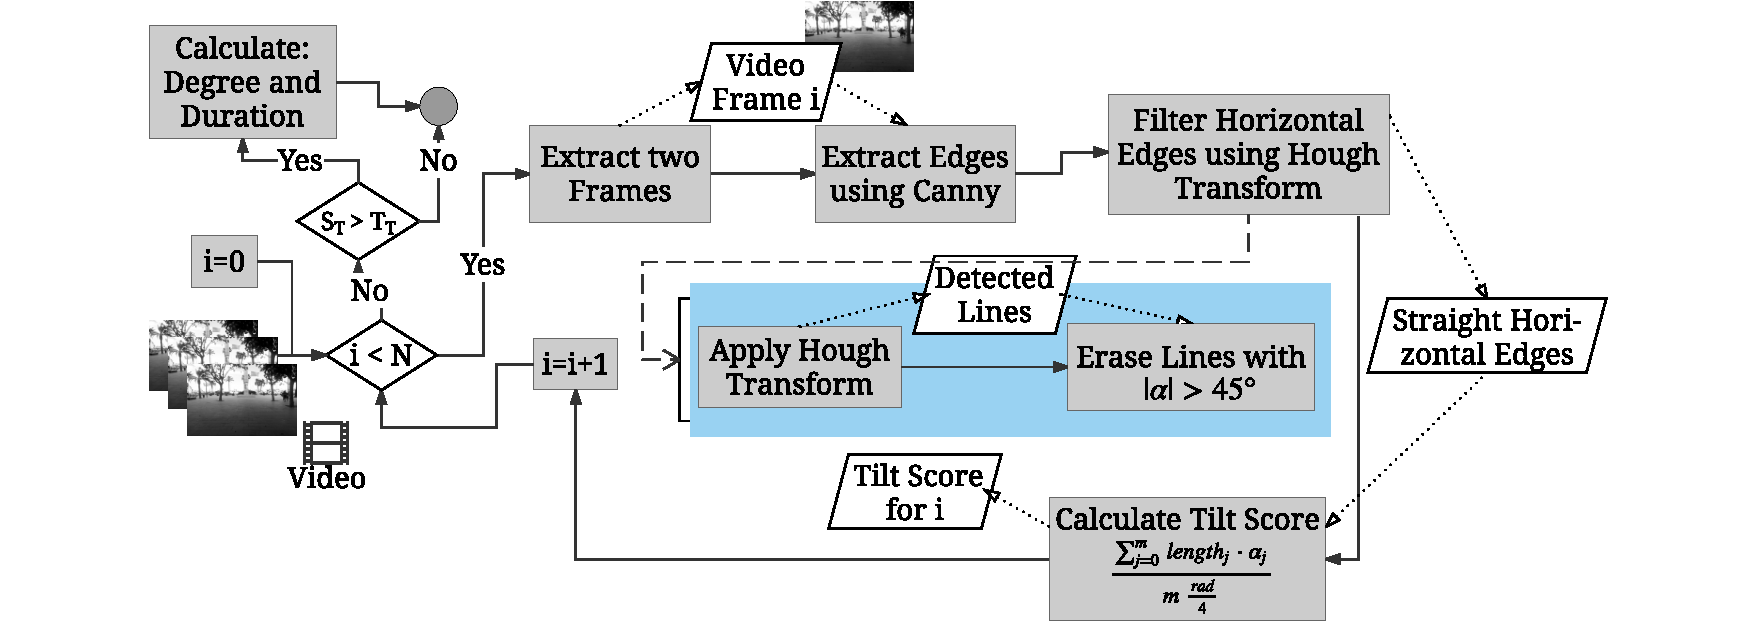
\includegraphics[width=\linewidth]{./gfx/550_QA/Tilt_algorithm_Video_based}
  	\caption[Video-based tilt detection]{Video-based camera tilt detection algorithm.} %; (b) Auxiliary sensor-based detection.} 
  	\label{fig:554_TiltDetection}
\end{figure} 
\subsubsection{Video-based Algorithm}
The algorithm as depicted in Figure~\ref{fig:554_TiltDetection} detects tilt in video recordings.
The algorithm extracts horizontal edges - or vertical ones in the case of a portrait-oriented recording - based on the Canny edge filter~\cite{Canny1986}, and determines straight lines using a Hough transform.
The Hough transform reduces the detected lines to those which are straight lines as contours of rectangular objects. 
Furthermore, straight horizontal lines are required, as only those allow for a reliable determination of an angle of the tilt to the horizontal plane.
In comparison to related approaches we do not require that the majority of edges in a video frame are horizontal edges~\cite{Saini2012}. 
Also, straight lines with an angle greater than $45\degree$ will be erased as they would misleadingly indicate a wrong orientation detected by the device.
In summary, straight horizontal lines do not need to be perfectly aligned with the horizontal plane, but should have an angle of less or equal $45\degree$ towards the plane.
Afterwards, an exact direction for each line is determined. 
In a final step, the tilt score (which is normalized $[0,1]$) is calculated by applying a calculation of the angle of a detected line to a perfect horizontal line as $\alpha$.
This angle is multiplied by the number of pixels of all horizontal lines and averaged.
Here, a measure close to 1 indicates long lines with a significantly tilted angle.
A threshold determines whether a tilt degrading the perceived quality is detected.
\subsubsection{Auxiliary Sensor-based Algorithm}
\paragraph{Tilt Detection}
An auxiliary sensor-based approach is proposed which relies on the accelerometer\footnote{The algorithm can be applied to the gyroscope, too. The reduced noise in the gyroscope samples and the higher sampling rate are not required for tilt detection. An disadvantage of the gyroscope is the higher energy footprint~\protect\cite{Koenig2013}.} in smart mobile devices.
The algorithm is straight-forward and leverages the x- ($a_x$) and y-components ($a_y$) of the acceleration to determine the angle the y-axis of the smart mobile device is rotated.
This angle determines the deviation to an undistorted reference.

A reference model is built to determine the initial orientation of the device ($O_D$). 
We determine the tilt in relation to this initial $O_D$.
Based on the difference of the global orientation of a device, the tilt is calculated as
\begin{equation}
\beta_{Tilt} = 
|\alpha_{Init} - \alpha|
\end{equation} 
where $\alpha$ is determined by $\alpha = arctan(\frac{a_x}{a_y})$.
$\alpha_{Init} = arctan(\frac{a_x}{a_y})$ is calculated in the first seconds of a video recording. 
We assume that these initial seconds of a video are captured without a degradation. 

A drawback of the accelerometer is its sensitivity to small movements and white noise. 
To improve the robustness, $\alpha_{Init}$ is calculated again after the recording device has moved. 
During a movement the hybrid algorithm does not use the auxiliary sensor-based subalgorithm but adapts to the video-based calculation.  
Also, a sample window of two seconds at a sampling rate of $4$ $\unit{Hz}$ is used and averaged for calculating the tilt angle.

A tilt that degrades the perceived quality is determined by $\beta_{Tilt}$ being larger than $T_{CM,AS}$.
$T_{CM,AS}$ represents the threshold that distinguishes tilts being transparent to the viewer and tilts representing a major degradation.
\paragraph{Collaborative Detection of Camera Misalignments}
\label{sec:554_misalignments}
To detect camera misalignment, we propose a collaborative sensing approach.
This approach is only applicable, if multiple recording devices record the same \ac{AoI}.
This scenario is illustrated in Figure~\ref{fig:554_fov}.
Here, all users except the red one are recording the \ac{AoI}.
We assume that the red user is recording an uninteresting part of a scene. As a simplification, the three-dimensional world is simplified to a two-dimensional model. 
A collaborative sensing approach is chosen to detect the \ac{AoI}. 
Our aim is to identify users who record non-interesting part of an event. 
The decision is solely based on the orientation and the \ac{FoV} of each recorder. 
Based on \ac{FoV} border lines, the intersection points of the \ac{FoV}s of all recording devices can be calculated. 
Majority voting is conducted on the most inner-lying intersection points of \ac{FoV} border lines, which are in the viewing direction of the recording devices.
\begin{figure}
	\centering
	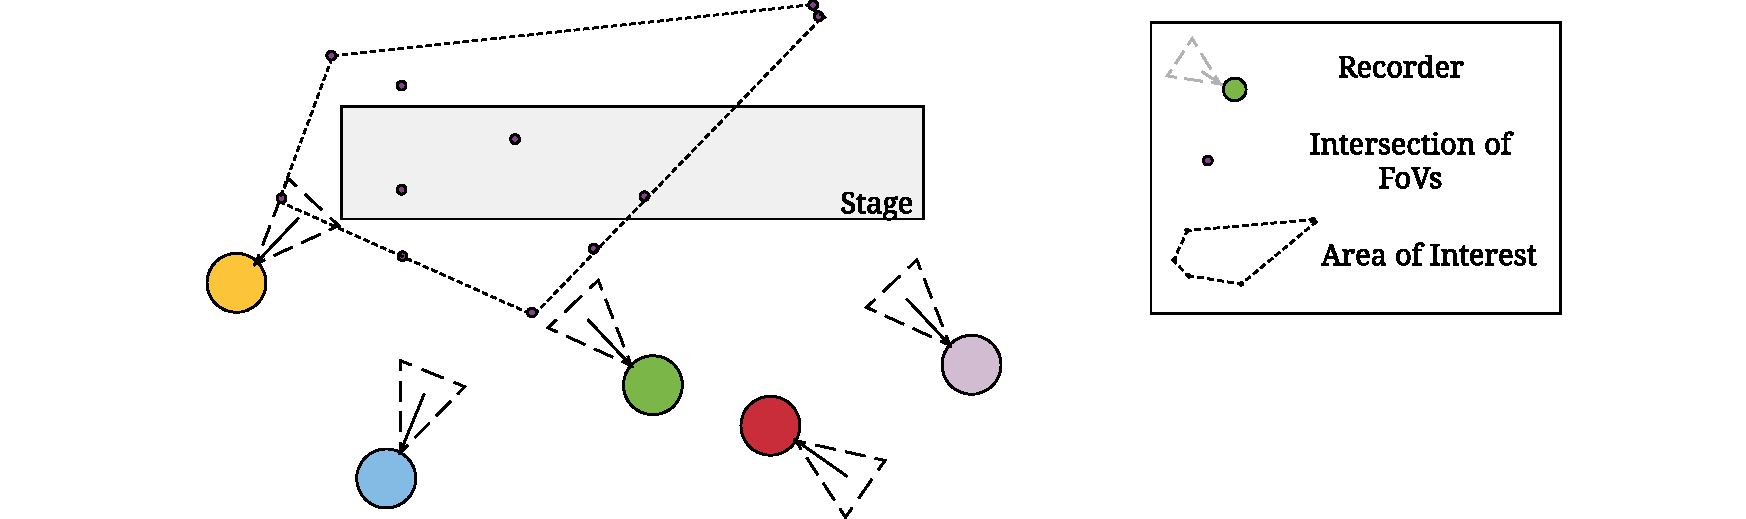
\includegraphics[width=\linewidth]{./gfx/550_QA/misalignment}
	\caption[Collaborative sensing for AoI detection.]{Collaborative sensing approach for eliminating views that do not record the \ac{AoI} of an event.}
	\label{fig:554_fov}
\end{figure}
The \ac{FoV} of each smart mobile device can be calculated based on the focal length $L_{F}$ as $FoV = 2 \times arctan(\frac{wi_{AS}}{2 \times  L_{F}})$, where $wi_{AS}$ represents the horizontal width of the sensor plane. 
Both parameters $L_{F}$ and the effective focal length $wi_{AS}$ are measured from EXIF tags from a captured photo on a smartphone. 
Also, the Android \ac{OS} offers an \ac{API} to retrieve the \ac{FoV} from camera parameters. 

For detecting the \ac{AoI}, a convex hull of the intersection points is applied where in-lying points are erased\footnote{
The basis for the calculations is the location data gathered from the \ac{GPS} that is mapped into a two-dimensional coordinate system based on the \ac{UTM}.}. 
For a quick calculation of the convex hull, the quick elimination approach ($O=N$) is used, which chooses a rectangle or quadrilateral of four points in the point set. 
Intersection points that are obviously non-feasible (large distance) % (greater than 500 meters) 
are discarded upfront.
Building the convex hull is achieved by using a Graham Scan~\cite{Graham1972}, which relies on a polar sorted list of  points. 
It starts at the lowest vertical point and systematically erases points which would result in a clockwise turn.

From the \ac{FoV}s of the recording devices, those video streams can be determined which do not record the common \ac{AoI}.
Furthermore, the deviation from the center of the \ac{AoI} is calculated, which allows to determine the characteristics of the quality model, as proposed in Section~\ref{sec:430_results_recording_degradations}.